\documentclass[a4paper,11pt]{article}
\usepackage{a4wide}
\usepackage{fullpage}
\usepackage[utf8x]{inputenc}

\usepackage[light,math]{anttor}
\usepackage[T1]{fontenc}

%\usepackage[slovene]{babel}
%\selectlanguage{slovene}
\usepackage[toc,page]{appendix}
\usepackage[pdftex]{graphicx} 

\usepackage{lmodern}
\usepackage{amsmath}
\usepackage{amssymb}
\usepackage{amsthm}
\usepackage{amsfonts}
\usepackage{mathtools}
\usepackage{enumitem}
\usepackage{amsfonts}
\usepackage{amsmath}
\usepackage{setspace}
\usepackage{color}
\definecolor{light-gray}{gray}{0.95}
\usepackage{listings} 
\usepackage{hyperref}
\usepackage{listings}

\renewcommand{\baselinestretch}{1.2} 
\renewcommand{\appendixpagename}{Priloge}


\title{Bayesova statistika \\
\textbf{Domača naloga 3} }
\author{Sara Bizjak  |  27202020}
\date{December 2021}

%%%%%%%%%%%%%%%%%%%%%%%%%%%%%%%%%%%%%%%%%%%%%%%%%%%%%%%%%%%%%%%%%%%%%%%%%%%%%%%%%%%%%%%%%%%%%%%%%%%%%%%%%%%%%%%%%%%%%%%%%%%%%%%%%

\begin{document}

\maketitle


\noindent
\textbf{1. naloga}
\\
Koda Gibbsovega vzorčevalnika. Kjer je kaj dodano ali spremenjeno iz kode iz vaj, je zraven komentar \texttt{DODANO} oz. \texttt{SPREMENJENO}.
Bolj pregledna koda (s klici za vse naslednje naloge) je dostopna v datoteki \texttt{DN3\_koda\_sarabizjak.R}.
\begin{lstlisting}
-------------------------------------------------------------------
# Uvoz podatkov:
setwd("~/Documents/ISRM magistrski/Bayesova statistika/BS/Domace naloge/DN3")
source("podatki_sole.R")
str(pod)

library(ggplot2)
ggplot(pod, aes(x = school, y = mathscore, group = school)) +
        stat_summary(fun.ymin = min, fun.ymax = max, fun.y = mean) + 
        labs(title = "Povprecja (pika) in razpon rezultatov po solah")

# Preureditev podatkov: 
library(dplyr)
pod.sole = pod %>%
    group_by(school) %>% 
    summarise(povprecje = mean(mathscore),
                        n=length(mathscore), 
                        varianca = var(mathscore))

# Nastavitev parametrov:

# Parametri (hiper)apriornih porazdelitev, isti kot na vajah:
sigma20 = 100
nu0 = 1
eta20 = 100
kappa0 = 1
mu0 = 50
tau20 = 25

# Parametri iz domace naloge: 
a = 2
b = 1 / 10
alpha = 2
k.max = 1000

### Pripravimo si kolicine, ki jih bomo potrebovali iz podatkov
x = pod
m = length(pod.sole$school) 
n = pod.sole$n
x.povpr = pod.sole$povprecje
x.var = pod.sole$varianca

### Dolocimo si zacetne vrednosti
muGroups = x.povpr
mu = mean(muGroups)
eta2 = var(muGroups)

# DODANO: shranimo sigmo za vsako skupino loceno
sigma2Groups = x.var 

### Pripravimo si prostor za shranjevanje
n.iter = 5000

muGroups.all = matrix(nrow = n.iter, ncol = m) 
mu.all = rep(NA, n.iter)
eta2.all = rep(NA, n.iter)

# DODANO:
sigma2Groups.all = matrix(nrow=n.iter, ncol= m)
sigma20.all = rep(NA, n.iter)
nu0.all = rep(NA, n.iter)

### Na prvo mesto si shranimo zacetne vrednosti (nepotrebno)
muGroups.all[1, ] = muGroups 
mu.all[1] = mu
eta2.all[1] = eta2

# DODANO: shranimo zacetne vrednosti novih parametrov
sigma2Groups.all[1,] = sigma2Groups
sigma20.all[1] = sigma20 
nu0.all[1] = nu0

### Pozenemo Gibbsov vzorcevalnik

set.seed(1)
for (s in 1 : n.iter) {
    
    # Vzorcimo muGroups
    for (j in 1 : m) {
    # SPREMENJENO: sigma2 v enacbi je zamenjana s sigma2Groups[j], 
    #              ostalo je enako
    muGroups[j] = rnorm(1,
                        mean = (x.povpr[j] * n[j] / sigma2Groups[j] + mu / eta2) / (n[j] / sigma2Groups[j] + 1 / eta2),
                        sd = sqrt(1 / (n[j] / sigma2Groups[j] + 1 / eta2)))
    }
    
    # DODANO: Vzorcimo sigma2Groups namesto sigma2, delamo po skupinah... 
    #         po formuli iz domace naloge
    for(j in 1 : m){
    sigma2Groups[j] = 1 / rgamma(1,
                                    (nu0 + n[j]) / 2,
                                    (nu0 * sigma20 + sum((x[x[, 1] == j, 2] - muGroups[j])^2)) / 2)
    }
    
    # DODANO: Vzorcimo sigma20... po formuli iz domace
    sigma20 = rgamma(1,
                    a + m * nu0 / 2,
                    b + nu0 * sum(1 / sigma2Groups) / 2)
    
    # Vzorcimo mu, ne spreminjamo nic
    mu <- rnorm(1,
                mean = (mean(muGroups) * m / eta2 + mu0 / tau20) / (m / eta2 + 1 / tau20),
                sd = sqrt(1 / (m / eta2 + 1 / tau20)))
    
    # Vzorcimo eta2, ne spreminjamo nic
    ss   <- kappa0 * eta20 + sum((muGroups - mu)^2)
    eta2 <- 1 / rgamma(1, (kappa0 + m) / 2, ss / 2)
    
    # DODANO: Vzorcimo nu0, koda kopirana iz navodil za domaco nalogo
    k <- 1:k.max
    logp.nu0 <- m * (0.5 * k * log(k*sigma20/2) - lgamma(k/2)) +
    (k/2-1) * sum(log(1/sigma2Groups)) +
    - k * (alpha + 0.5 * sigma20 * sum(1/sigma2Groups))
    nu0 <- sample(k, 1, prob = exp(logp.nu0 - max(logp.nu0)))
    
    # Shranimo nove parametre
    muGroups.all[s,] = muGroups 
    mu.all[s] = mu
    eta2.all[s] = eta2
    
    # DODANO:
    sigma2Groups.all[s,] = sigma2Groups
    sigma20.all[s] = sigma20 
    nu0.all[s] = nu0
}
-------------------------------------------------------------------
\end{lstlisting}


\noindent
\textbf{2. naloga: Proučevanje konvergence}

\begin{figure}[ht!]
    \centering
    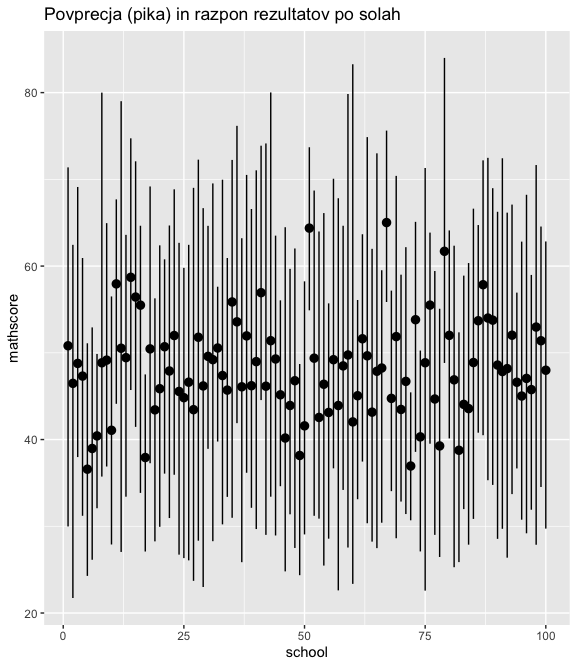
\includegraphics[width = 95mm]{Slike/naslovna.png}
    \caption{Podatki šol.}
\end{figure}
\noindent
\textit{Trace plots.}
\\
Poglejmo si najprej trace plots za hiperparametre.

\begin{figure}[ht!]
    \centering
    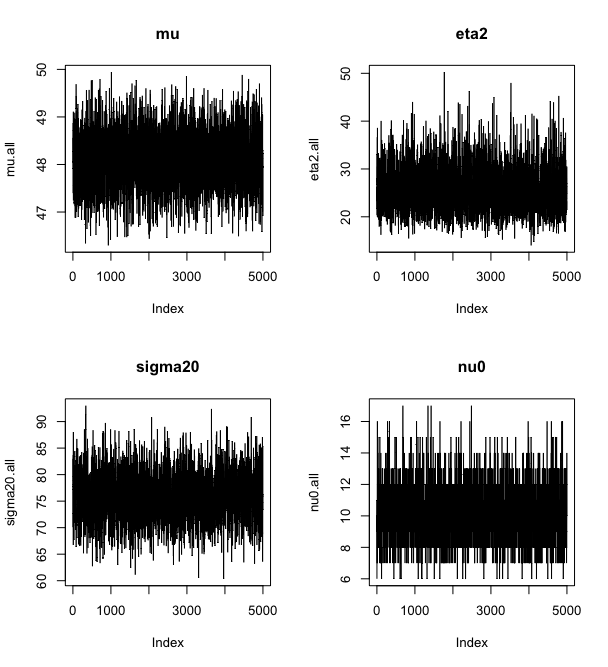
\includegraphics[width = 150mm]{Slike/2_hiper.png}
    \caption{Trace plots za hiperparametre.}
\end{figure}
\noindent
Videti je, da je kovergenca dosežena, zaporedje pa se že takoj giba v območju porazdelitve, tako da \textit{burn-in} ni potreben. 
Rezultat je pričakovan, saj smo za začetno vrednost zaporedja izbrali vzorčno povprečje posamezne skupine (oz. vzorčno varianco), kar je najbolj možna smiselna začetna vrednost.

\newpage
Poglejmo si še iste grafe z izrisanimi prvimi 500 členi zaporedij.

\begin{figure}[ht!]
    \centering
    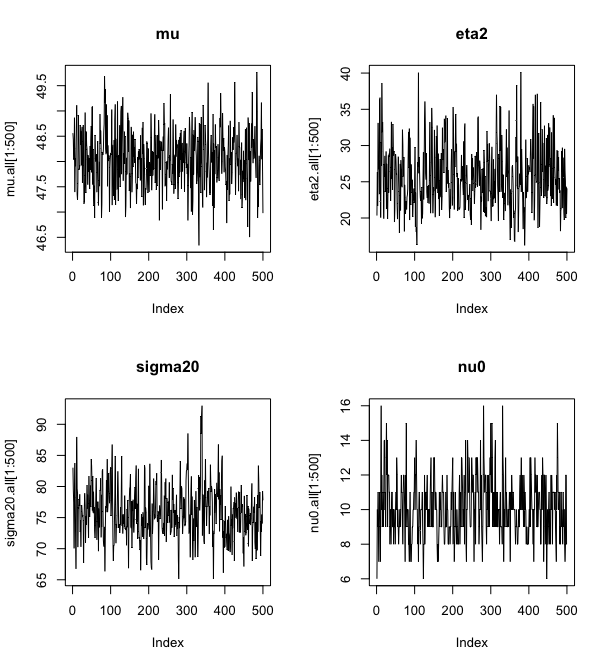
\includegraphics[width = 150mm]{Slike/2_hiper_500.png}
    \caption{Trace plots za hiperparametre z izrisanimi prvimi 500 členi zaporedij.}
\end{figure}

\noindent
Slednji grafi s 500 členi zaporedij samo še potrdijo prejšnjo trditev o \textit{burn-in} parametru, katerega res ne potrebujemo.
Iz grafa za $nu0$ se zazdi, da so vrednosti diskretne. Izpis dejanskih vrednsti domnevo potrdi.

\newpage
Poglejmo še ostale parametre, (naključno) si izberemo šole $j = 1, 10, 50, 80$.


\begin{figure}[ht!]
    \centering
    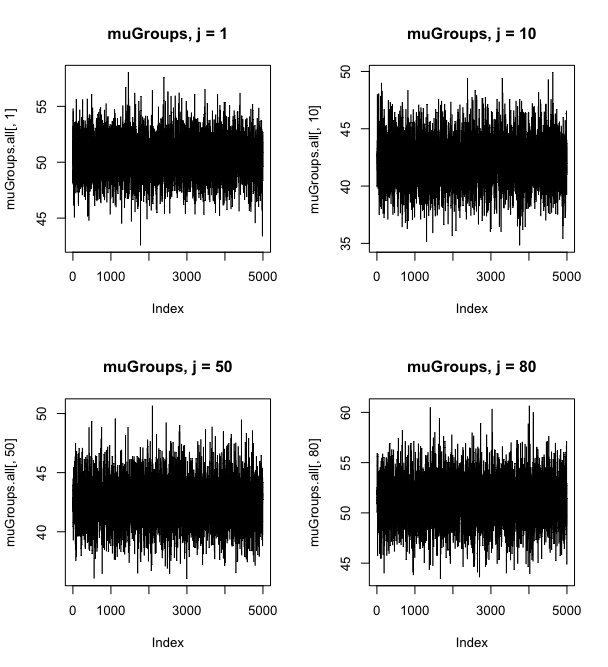
\includegraphics[width = 150mm]{Slike/2_muGroups.png}
    \caption{Trace plots za parameter \texttt{muGroups}.}
\end{figure}
\newpage
\begin{figure}[ht!]
    \centering
    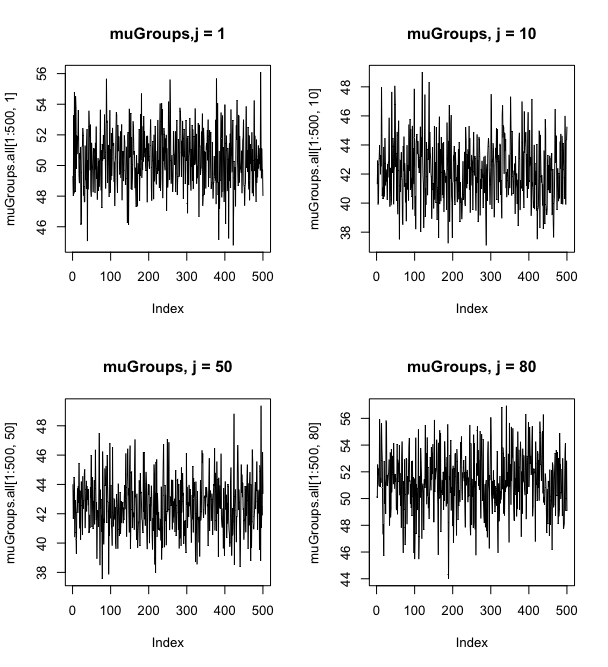
\includegraphics[width = 150mm]{Slike/2_muGroups_500.png}
    \caption{Trace plots za parameter \texttt{muGroups} z izrisanimi prvimi 500 členi zaporedja.}
\end{figure}
\newpage
\begin{figure}[ht!]
    \centering
    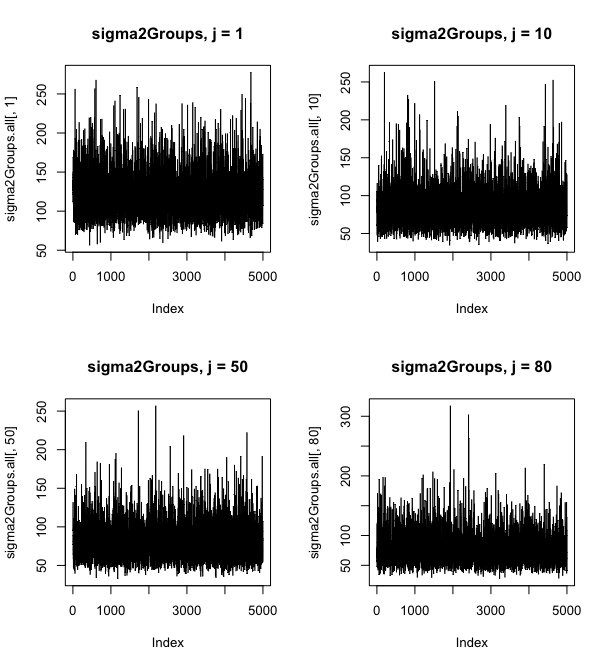
\includegraphics[width = 150mm]{Slike/2_sigma2Groups.png}
    \caption{Trace plots za parameter \texttt{sigma2Groups}.}
\end{figure}
\newpage
\begin{figure}[ht!]
    \centering
    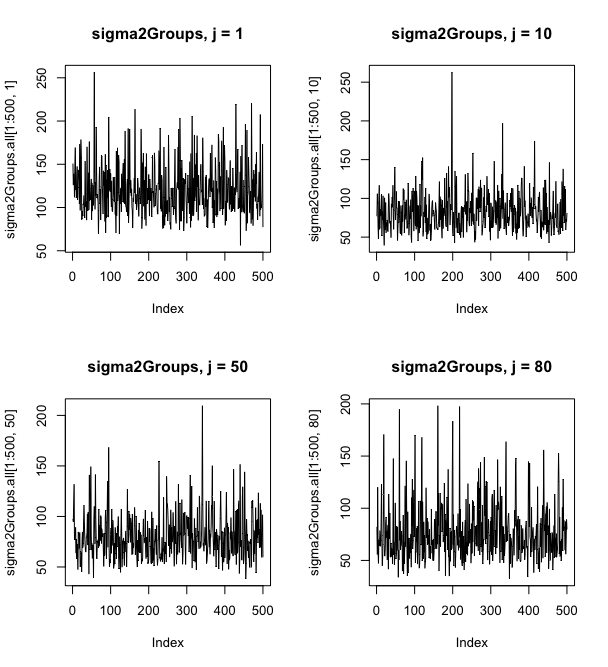
\includegraphics[width = 150mm]{Slike/2_sigma2Groups_500.png}
    \caption{Trace plots za parameter \texttt{sigma2Groups} z izrisanimi prvimi 500 členi zaporedja.}
\end{figure}
\noindent
Tudi pri teh parametrih, podobno kot pri hiper, ni videti \textit{burn-in} dela, zato povsod ohranimo celotne verige.
\\
\\
\textit{Porazdelitev vzorcev.}
\\
Za opazovanje porazdelitve vzorcev verigo razdelimo na desetine, torej na 10 enakih delov. 
V nadaljevanju potem za vsak podvzorec posebej opazimo povprečja (oz. variance) z intervali zaupanja, ki se morajo, za stabilnost verig, znotraj posamezne skupine relativno ujemati -- 
za stabilnost se torej znotraj posameznih podvzorcev povprečja \textit{lahko} razlikujejo, skozi vse podvzorce posamezne skupine pa se morajo "gibati v istem rangu".
Izrišimo sedaj grafe, da bo jasno, kaj smo s tem mislili.
\newpage
\begin{figure}[ht!]
    \centering
    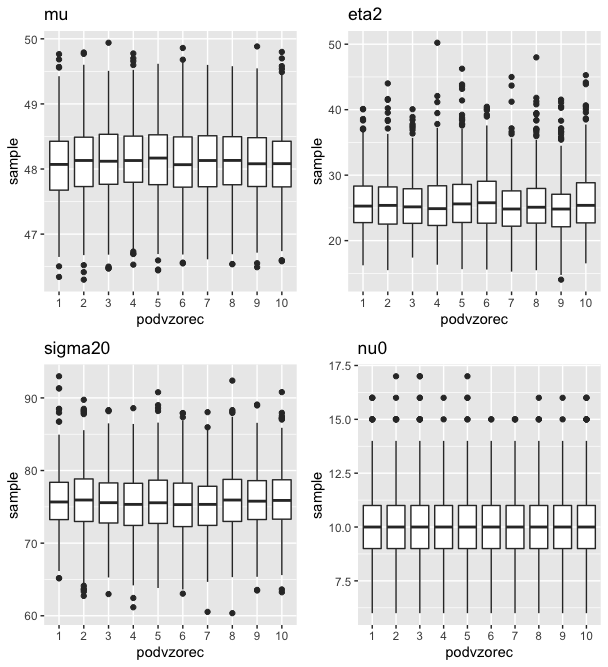
\includegraphics[width = 150mm]{Slike/vzorci_hiper.png}
    \caption{Porazdelitev podvzorcev za hiperparametre.}
\end{figure}
\newpage
\begin{figure}[ht!]
    \centering
    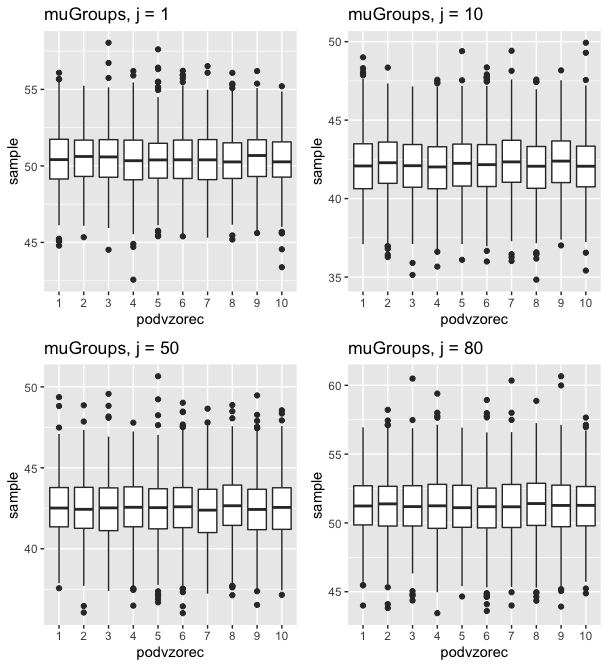
\includegraphics[width = 150mm]{Slike/vzorci_muGroups.png}
    \caption{Porazdelitev podvzorcev za parameter \texttt{muGroups}.}
\end{figure}
\newpage
\begin{figure}[ht!]
    \centering
    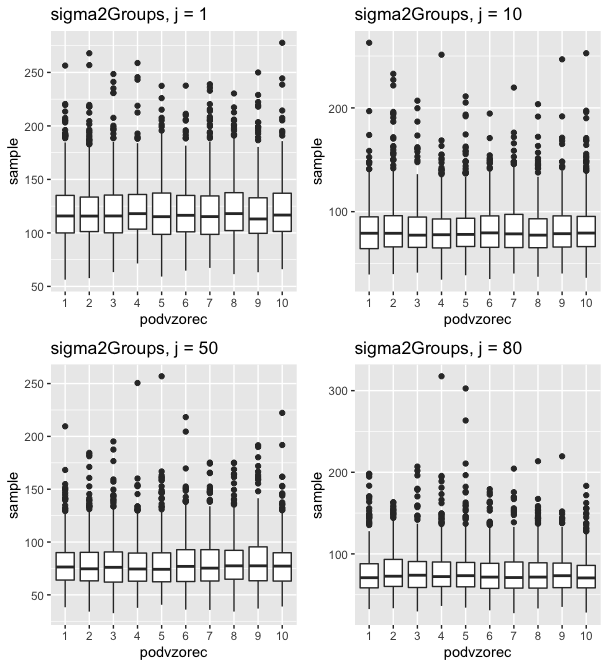
\includegraphics[width = 150mm]{Slike/vzorci_sigma2Groups.png}
    \caption{Porazdelitev podvzorcev za parameter \texttt{sigma2Groups}.}
\end{figure}

\noindent
Iz grafov razberemo, da so verige stabilne. Generalno gledano so med posameznimi skupinami, tj.~šolami, opazne manjše razlike, znotraj skupine pa so podvzorci stabilni.
Imamo torej situacijo, kot smo jo opisali že zgoraj.

\newpage
\noindent
\textit{Avtokorelacije.}
\\
Poglejmo si še avtokorelacije. Najprej za hiperparametre in potem še za nekaj ostalih.
\begin{figure}[ht!]
    \centering
    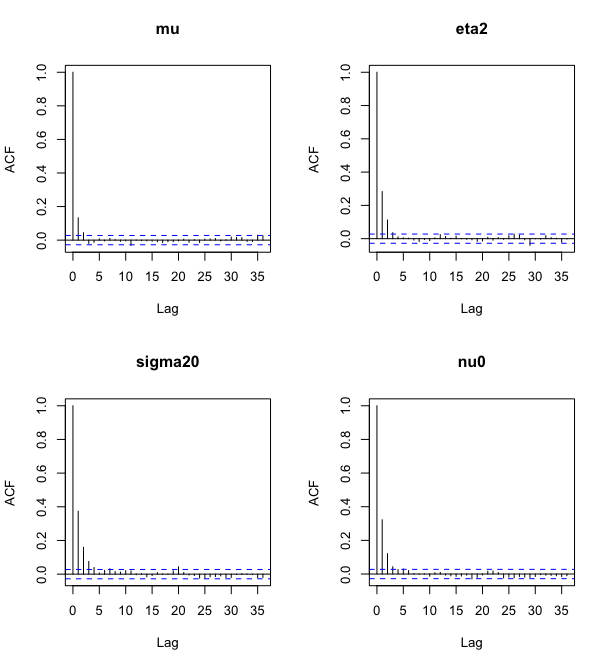
\includegraphics[width = 160mm]{Slike/avto_hiper.png}
    \caption{Avtokorelacije za hiperparametre}
\end{figure}
\newpage
\begin{figure}[ht!]
    \centering
    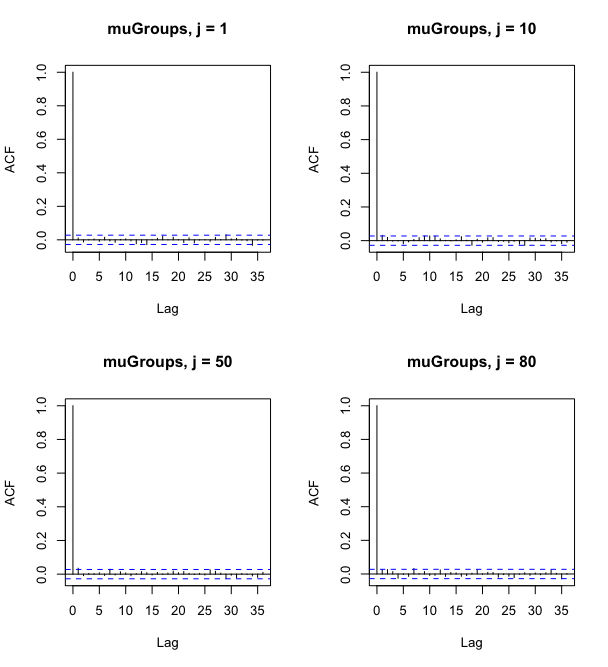
\includegraphics[width = 160mm]{Slike/avto_muGroups.png}
    \caption{Avtokorelacije za parameter \texttt{muGroups}.}
\end{figure}
\newpage
\begin{figure}[ht!]
    \centering
    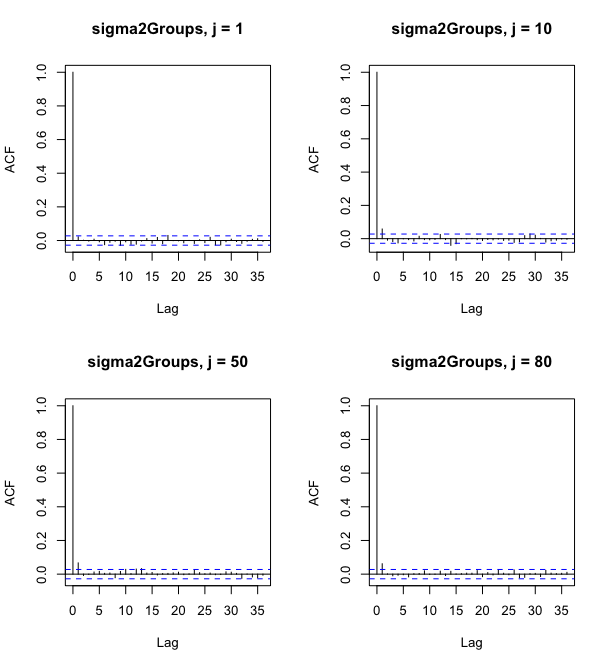
\includegraphics[width = 160mm]{Slike/avto_sigma2Groups.png}
    \caption{Avtokorelacije za parameter \texttt{sigma2Groups}.}
\end{figure}

\noindent
Opazimo, da v splošnem ni težav z avtokorelacijo. Omenimo le, da je pri hiperharametrih opazno, da se avtokorelacija malce kasneje približa 0 (pri zamiku 1 je avtokorelacije po definiciji 1, zato je na začetku povsod tam).
\\
Poglejmo sedaj še naslednje izračune, ki so povezani z avtokoreliranostjo.

\newpage
\noindent
\textit{Effective sample size.}
\\
\textit{Effective sample size} nam pove, za koliko n.e.p. je naš vzorec "vreden".

\begin{itemize}
    \item Hiperparametri:
        \begin{itemize}
            \item \texttt{mu: 3841.048}
            \item \texttt{eta2: 2604.908}
            \item \texttt{sigma20: 2181.228}
            \item \texttt{nu0: 2563.581 }
        \end{itemize}
    \item muGroups:
        \begin{itemize}
            \item \texttt{j = 1: 5000 }
            \item \texttt{j = 10: 4698.121 }
            \item \texttt{j = 50: 4662.577 }
            \item \texttt{j = 80: 4484.269 }
        \end{itemize}
    \item sigma2Groups:
        \begin{itemize}
            \item \texttt{j = 1: 4788.897}
            \item \texttt{j = 10: 4452.038}
            \item \texttt{j = 50: 4374.3 }
            \item \texttt{j = 80: 4419.596 }
        \end{itemize}
\end{itemize}

\noindent
Takoj opazimo, da je \textit{Effective sample size} pri hiperparametrih, kjer je bila opažena tudi malenkost slabša korelacija, nižji, kot pri ostalih.
\textit{Effective sample size} je torej višji pri parametih z višjo avtokorelacijo in obratno.

\newpage
\noindent
\textbf{3. naloga: Marginalne aposteriorne porazdelitve}
\\
Poglejmo si marginalne aposteriorne porazdelitve za hiperparametre in nekaj ostalih parametrov (podobno kot prej za $j = 1, 10, 50, 80$).

\begin{figure}[ht!]
    \centering
    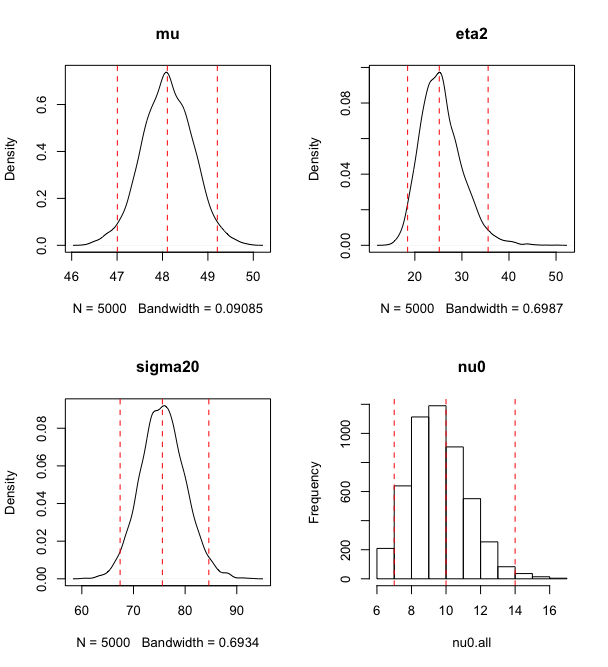
\includegraphics[width = 160mm]{Slike/3_hiper.png}
    \caption{Marginalne aposteriorne porazdelitve za hiperparametre.}
\end{figure}
\noindent
Opazimo, da je graf za parameter \texttt{mu} simetričen in normalno porazdeljen. 
\\
Podobno bi lahko trdili tudi za parameter \texttt{sigma20}, pa čeprav vemo, da je vzorčen iz gama porazdelitve. 
Ker pa gama porazdelitev pri dovolj velikih parametrih konvergira k normalni (oz. jo lahko aproksimiramo z normalno porazdelitvijo), je rezultat in grafika tukaj smiselna.
\\
Parameter \texttt{eta2} je nekoliko asimetričen, ker izhaja iz inverzne gamma porazdelitve.
\\
Ker ima \texttt{nu0} diskretne vrednosti, je njegova porazdelitev prikazan s histogramom. Opazimo, da je nekoliko asimetričen oz. nagnjen v levo.
\\
Zapišimo še intervale zaupanja (označeno z rdečo) v zaporedju kot jih izpiše \texttt{R (2.5\%       50\%     97.5\%)}:
\begin{itemize}
    \item \texttt{mu: 47.00592 48.10700 49.20768 }
    \item \texttt{eta2: 8.46046 25.18481 35.56685}    
    \item \texttt{sigma20: 67.40757 75.59166 84.58613 }
    \item \texttt{nu0: 7    10    14  }
\end{itemize}

\newpage
\begin{figure}[ht!]
    \centering
    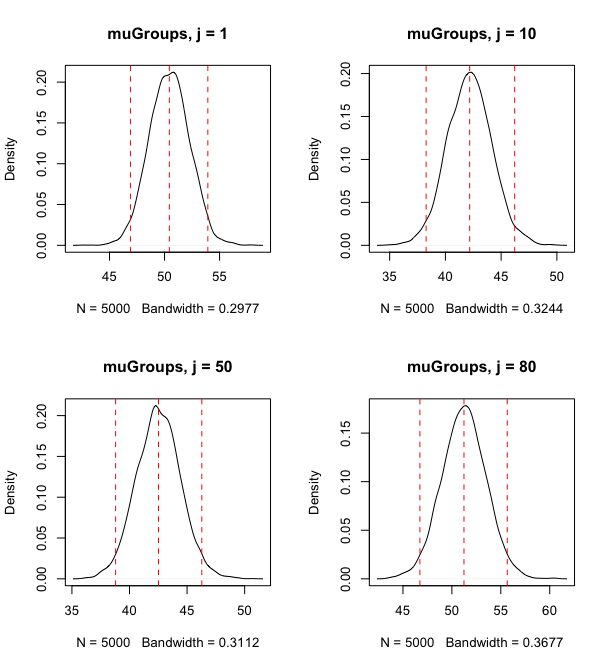
\includegraphics[width = 150mm]{Slike/3_muGroups.png}
    \caption{Marginalne aposteriorne porazdelitve za parameter \texttt{muGroups}.}
\end{figure}
\noindent
Grafi porazdelitev izgledajo po pričakovanjih, saj smo jih vzorčili iz normalne porazdelitve -- zato izgledajo normalno porazdeljeni, simetrični.
\\
Zapišimo še intervale zaupanja (označeno z rdečo) v zaporedju kot jih izpiše \texttt{R (2.5\%       50\%     97.5\%)}:
\begin{itemize}
    \item \texttt{muGroups, j = 1: 46.90124 50.43449 53.93451  }
    \item \texttt{muGroups, j = 10: 38.27189 42.17707 46.21525  }
    \item \texttt{muGroups, j = 50: 38.79428 42.51917 46.27882  }
    \item \texttt{muGroups, j = 80: 46.72947 51.23621 55.65984  }
\end{itemize}

\newpage
\begin{figure}[ht!]
    \centering
    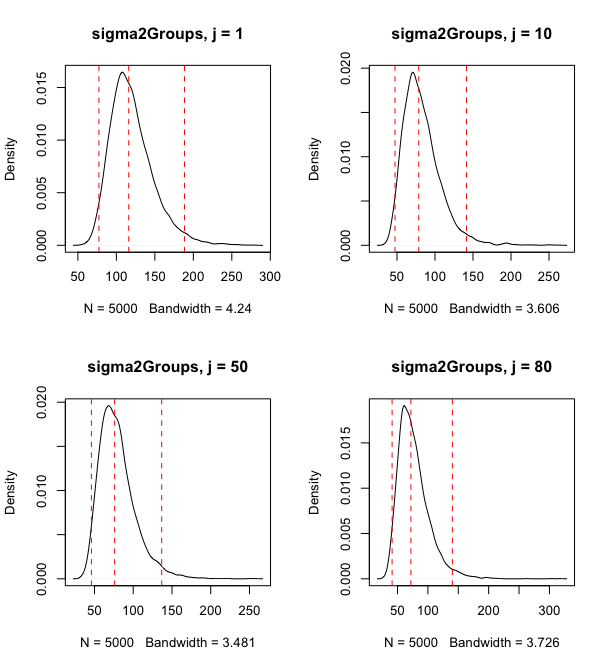
\includegraphics[width = 150mm]{Slike/3_sigma2Groups.png}
    \caption{Marginalne aposteriorne porazdelitve za parameter \texttt{sigma2Groups}.}
\end{figure}
\noindent
Tudi tukaj so rezultati pričakovani. Opazimo asimetričnost porazdelitev, kar je pričakovano, saj vzorčimo iz inverzne gamma porazdelitve.
\\
Zapišimo še intervale zaupanja (označeno z rdečo) v zaporedju kot jih izpiše \texttt{R (2.5\%       50\%     97.5\%)}:
\begin{itemize}
    \item \texttt{sigma2Groups, j = 1: 77.31629 116.05267 188.50244 }
    \item \texttt{sigma2Groups, j = 10: 47.39666  78.63839 141.44978 }
    \item \texttt{sigma2Groups, j = 50: 46.05211  76.02615 136.74937 }
    \item \texttt{sigma2Groups, j = 80: 41.14931  72.06370 140.34279  }
\end{itemize}
\noindent
Še splošen komentar:
\\
Iz zadjih dveh sklopov grafov (za \texttt{muGroups} in \texttt{sigma2Groups}) razberemo povprečje oz. varianco ocen matematike za posamezne šole, zato si jih lahko interpretiramo kot prikaz uspešnosti posamezne šole na področju matematike.
\\
\\
\noindent
\textbf{4. naloga: Shrinkage}
Poglejmo si najprej \textit{shrinkage} za povprečja.
\begin{figure}[ht!]
    \centering
    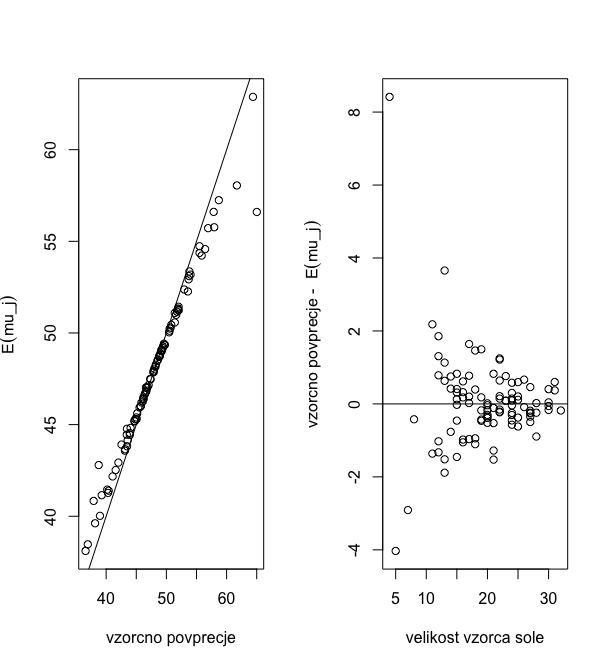
\includegraphics[width = 150mm]{Slike/4_povpr.png}
    \caption{\textit{Shrinkage} za povprečja.}
\end{figure}

\noindent
Lepo se vidi \textit{shrinkage} efekt. 
Opazimo, da so skupine, ki bolj odstopajo od povprečja, veliko bolj skrčene k skupnemu povprečju.
Na desni sliki opazimo, da je za skupine z manjšim vzorcem (velikost vzorca šol) premik večji, za večje skupine pa manj (bolj verjamemo večjim skupinam).
To je zato, ker pri šoli z manjšim vzorvem lahko bolj zgrešimo povprečje šole in zato bolj verjamemo skupnemu povprečju kor pa njenemu vzorčnemu povprečju -- zato se k skupnemu povprečju bolj približamo/premaknemo kot pa pri večjih šolah.
\\
Podobno poglejmo še za variance.

\begin{figure}[ht!]
    \centering
    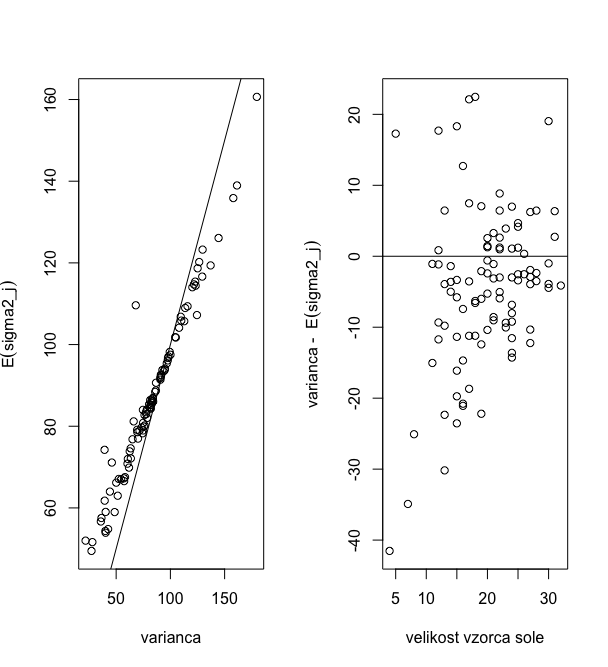
\includegraphics[width = 150mm]{Slike/4_var.png}
    \caption{\textit{Shrinkage} za variance.}
\end{figure}
\noindent
Tukaj lahko rečemo podobno, sploh za prvo sliko. Če si pa ogledamo drugo sliko, bi lahko rekli, da velikost skupine ne vpliva toliko na skrčenje variance kot pri prejšnjem primeru s povprečji, je pa to še vedno moč opaziti.

\newpage
\noindent
\textbf{5. naloga: Primerjava z modelom iz vaj}
\\
Če naš model primerjamo z modelom iz vaj, pri rezultatih ne opazimo večjih razlik.
\\
Z dodajanjem variance za posamezne skupine nismo konkretno prispevali k porazdelitvam. 
Kljub temu, da z dodajanjem variance prinesemo dodatno informacijo o šolah (teh informacij prej nismo imeli, saj smo predpostavljali enake variance), pa vpeljava različnih varianc za naše podatke k temu modelu ni bila potrebna.
\\
\\
Kater model se odločimo uporabiti je seveda odvisno od veliko dejavnikov. Če bi imeli npr. veliko podatkov, informacija o posameznih variancah pa ne bi prispevala dodatnega znanja (ali pa da bi nas zanimala samo povprečja), potem bi uporabila model iz vaj.
Po drugi strani pa ta model iz domače naloge ni veliko bolj časovno zahteven, zato bi, če bi nam informacija o variancah koristila in prispevala koristna znanja, uporabili ta model.
\\
Zaključimo torej, da za naše podatke iz te domače naloge ne bi (nujno) potrebovali modela z različnimi variancami -- po drugi strani nas pa ne stane veliko več časa, saj podatkov ni veliko. Tako da bi se lahko odločili za oboje, rezultati pa bi bili podobno interpretativni v obeh primerih.

\end{document}